%%%%%%%%%%%%%%%%%%%%%%%%%%%%%%%%%%%%%%%%%%%%%%%%%%%%%%%%%%%%%%%%
%%%%%%%%%%%%%%%%%%%%%%%%%%%%%%%%%%%%%%%%%%%%%%%%%%%%%%%%%%%%%%%%
%%%%
%%%% This text file is part of the source of 
%%%% `Introduction to High-Performance Scientific Computing'
%%%% by Victor Eijkhout, copyright 2012-6
%%%%
%%%% This book is distributed under a Creative Commons Attribution 3.0
%%%% Unported (CC BY 3.0) license and made possible by funding from
%%%% The Saylor Foundation \url{http://www.saylor.org}.
%%%%
%%%%
%%%%%%%%%%%%%%%%%%%%%%%%%%%%%%%%%%%%%%%%%%%%%%%%%%%%%%%%%%%%%%%%
%%%%%%%%%%%%%%%%%%%%%%%%%%%%%%%%%%%%%%%%%%%%%%%%%%%%%%%%%%%%%%%%

The idea behind a
pipeline is as follows. Assume that an operation consists of multiple
simpler operations, and that for each suboperation there is separate
hardware in the processor.
For instance, an addition instruction can have the following components:
\begin{itemize}
\item Decoding the instruction, including finding the locations of the
  operands.
\item Copying the operands into registers (`data fetch').
\item Aligning the exponents; the addition
  %
  $.35\times 10^{-1}\,+\, .6\times 10^{-2}$ becomes 
  %
  $.35\times 10^{-1}\,+\, .06\times 10^{-1}$.
\item Executing the addition of the mantissas, in this case giving 
  %
  $.41$.
\item Normalizing the result, in this example to $.41\times
  10^{-1}$. (Normalization in this example does not do anything. Check
  for yourself that in 
  %
  $.3\times10^0\,+\,.8\times 10^0$ and 
  % 
  $.35\times10^{-3}\,+\,(-.34)\times 10^{-3}$ there is a non-trivial
  adjustment.)
\item Storing the result.
\end{itemize}
These parts are often called the `stages' or `segments' of the pipeline.

If every component is designed to finish in 1 clock cycle, the whole
instruction takes 6~cycles. However, if each has its own hardware, we
can execute two operations in less than 12~cycles:
\begin{itemize}
\item Execute the decode stage for the first operation;
\item Do the data fetch for the first operation, and at the same time
  the decode for the second.
\item Execute the third stage for the first operation and the second
  stage of the second operation simultaneously.
\item Et cetera.
\end{itemize}
You see that the first operation still takes 6 clock cycles, but the
second one is finished a mere 1~cycle later. 

Let us make a formal analysis of the speedup you can get from a
pipeline. On a traditional \ac{FPU}, producing $n$ results
takes $t(n)=n\ell\tau$ where $\ell$~is the number of stages, and
$\tau$~the clock cycle time. The rate at which results are produced is
the reciprocal of $t(n)/n$: $r_{\mathrm{serial}}\equiv(\ell\tau)\inv$.

On the other hand, for a pipelined \ac{FPU} the time is
$t(n)=[s+\ell+n-1]\tau$ where $s$ is a setup cost:
the first operation still has to go through the same stages
as before, but after that one more result will be
produced each cycle. We can also write this formula as\index{n@$n_{1/2}$}
\[ t(n)=[n+n_{1/2}]\tau, \]
expressing the linear time, plus an offset.


\begin{figure}[ht]
  \begin{quote}
  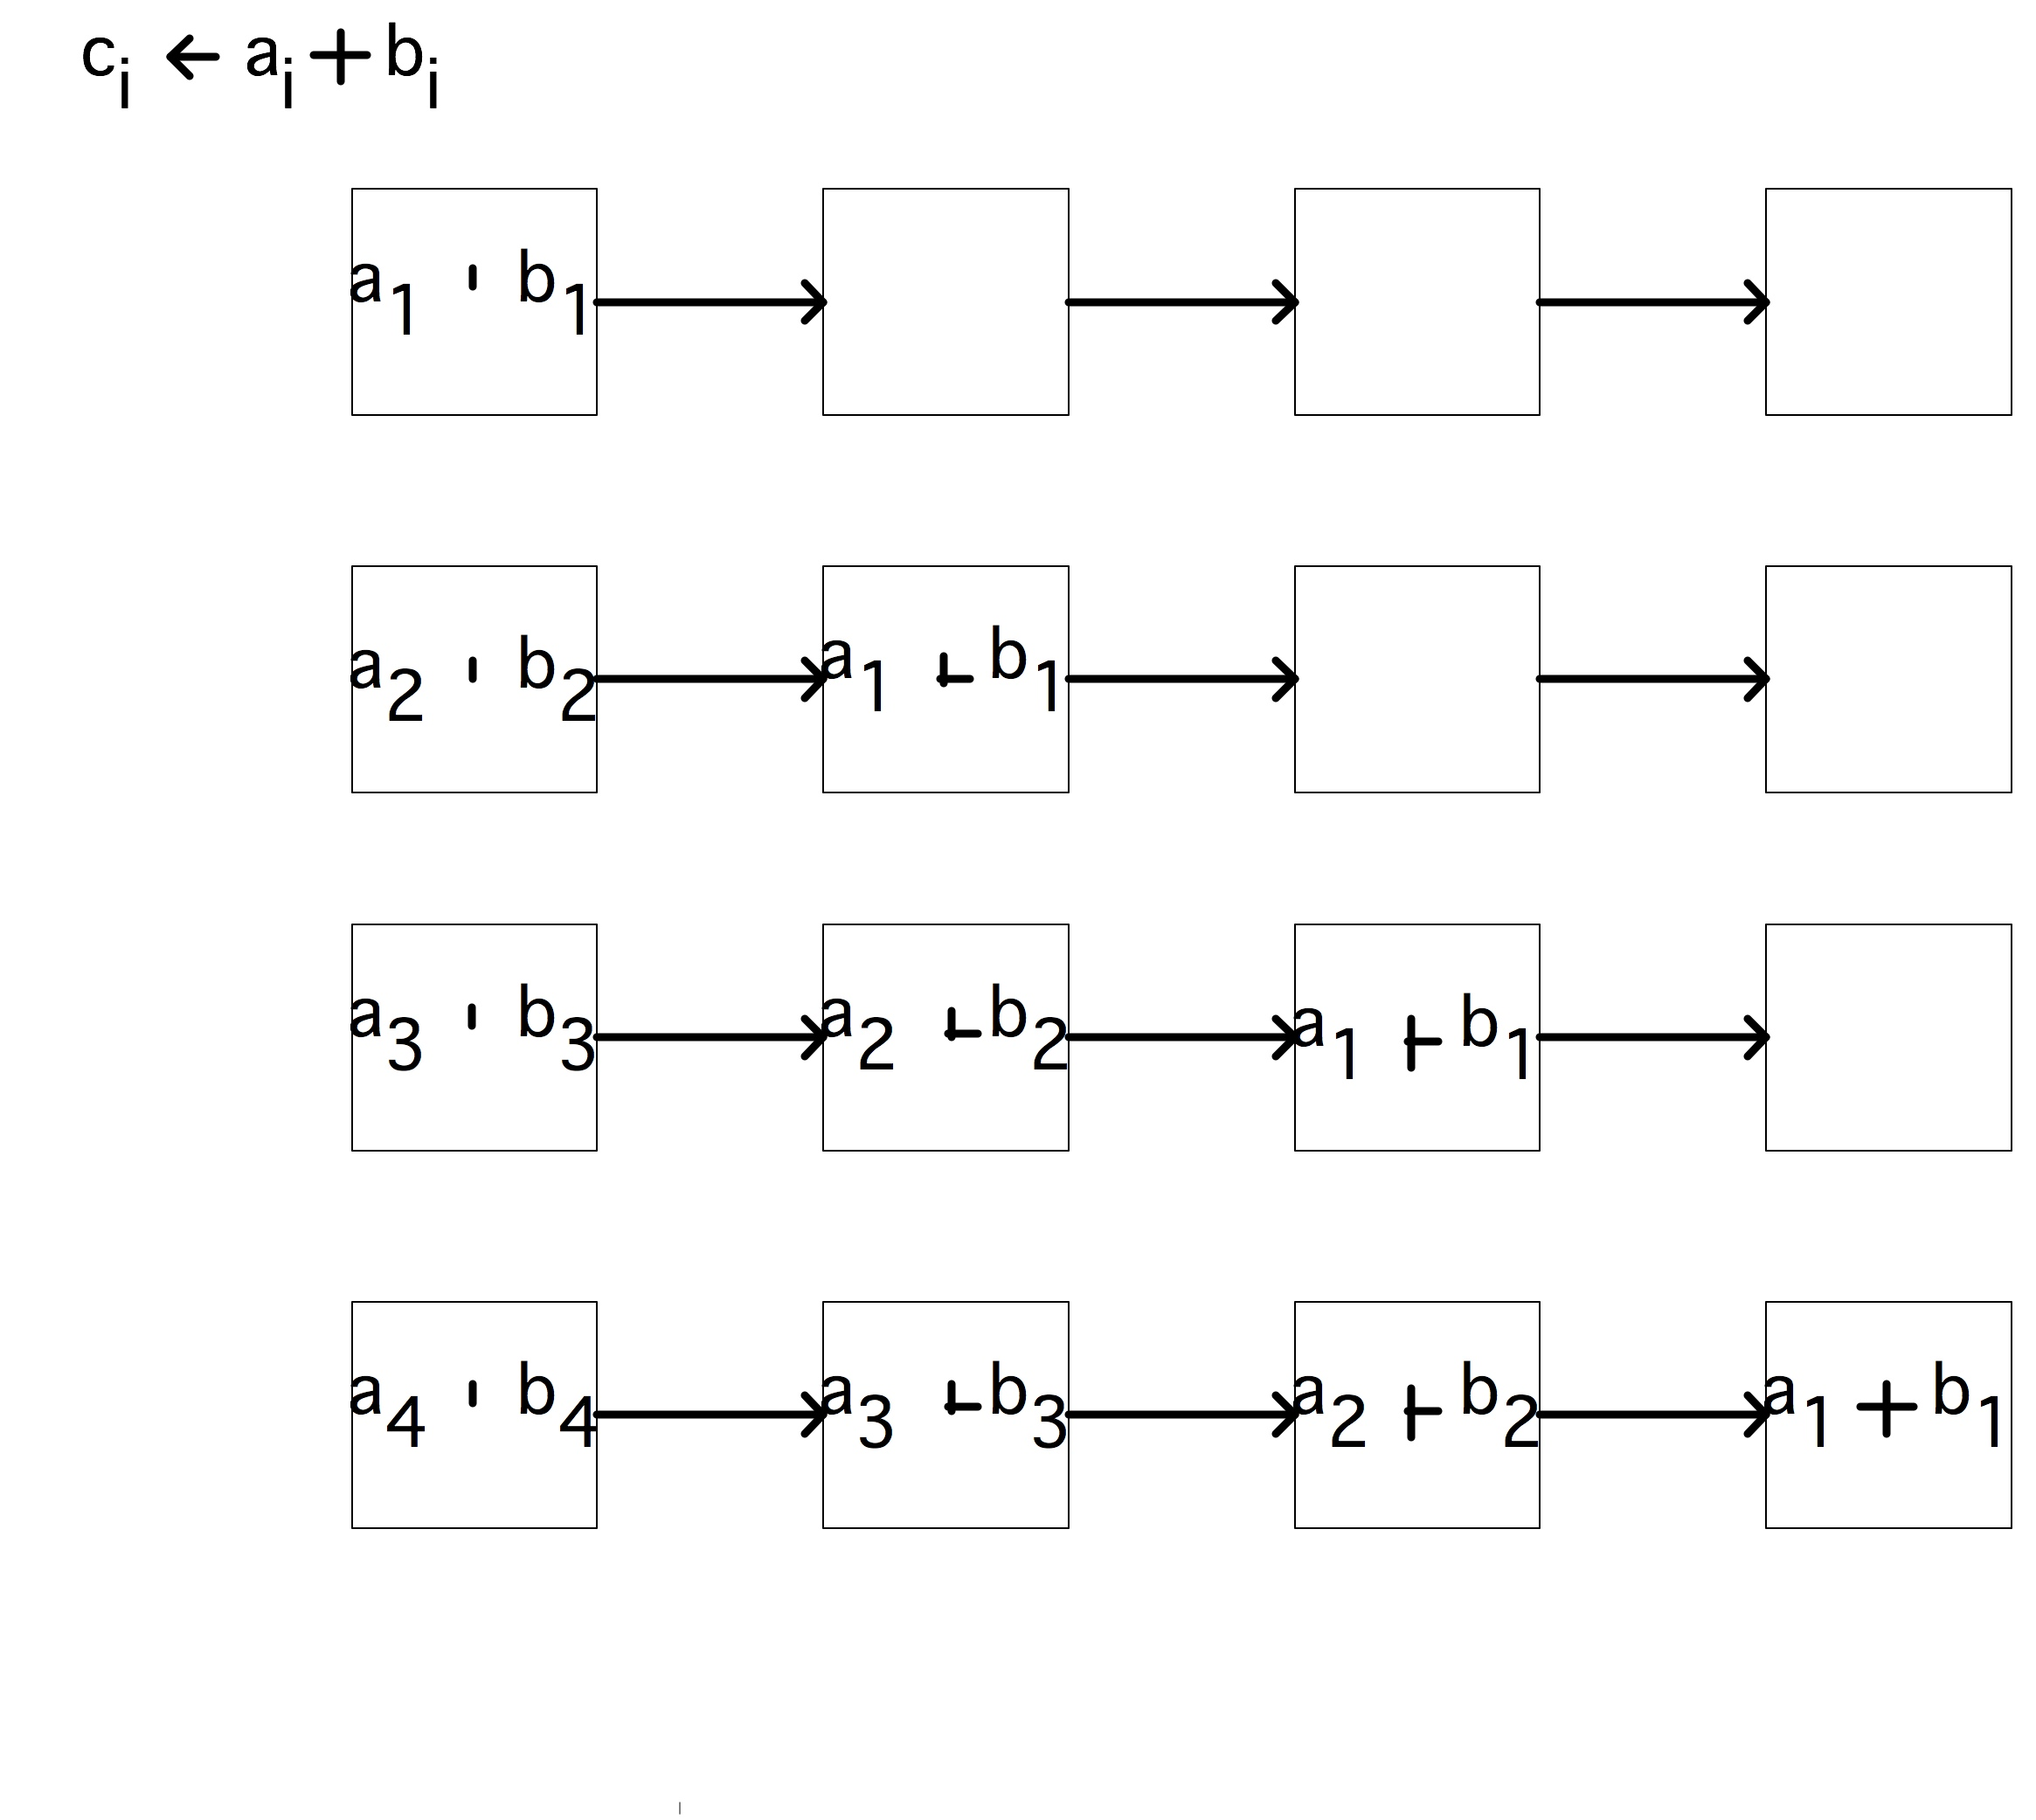
\includegraphics[scale=.12]{graphics/pipeline}
  \end{quote}
  \caption{Schematic depiction of a pipelined operation}
  \label{fig:pipeline}
\end{figure}
\begin{exercise}
  Let us compare the speed of a classical \ac{FPU}, and a pipelined
  one. Show that the result rate is now dependent on~$n$: give a
  formula for $r(n)$, and for
  $r_\infty=\lim_{n\rightarrow\infty}r(n)$. What is the asymptotic
  improvement in $r$ over the non-pipelined case?

  Next you can wonder how long it takes to get close to the asymptotic
  behaviour. Show that for $n=n_{1/2}$ you get $r(n)=r_\infty/2$.
  This is often used as the definition of~$n_{1/2}$.
\end{exercise}
Since a vector processor works on a number of instructions
simultaneously, these instructions have to be independent. The
operation $\forall_i\colon a_i\leftarrow b_i+c_i$ has independent
additions; the operation $\forall_i\colon a_{i+1}\leftarrow
a_ib_i+c_i$ feeds the result of one iteration ($a_i$) to the input of
the next ($a_{i+1}=\ldots$), so
the operations are not independent. 
%% In this respect,
%% a vector processor is like an array processor, and for this reason,
%% pipelines are often characterized as SIMD processors.

A pipelined processor can speed up operations by a factor of $4,5,6$
with respect to earlier CPUs. Such numbers were typical in the 1980s
when the first successful vector computers came on the market. These
days, CPUs can have 20-stage pipelines. Does that mean they are
incredibly fast? This question is a bit complicated. Chip designers
continue to increase the clock rate, and the pipeline segments can no
longer finish their work in one cycle, so they are further split
up. Sometimes there are even segments in which nothing happens: that
time is needed to make sure data can travel to a different part of the
chip in time.


The amount of improvement you can get from a pipelined CPU is limited,
so in a quest for ever higher performance several variations on the
pipeline design have been tried. For instance, the Cyber 205 had
separate addition and multiplication pipelines, and it was possible to
feed one pipe into the next without data going back to memory
first. Operations like $\forall_i\colon a_i\leftarrow b_i+c\cdot d_i$
were called `linked triads' (because of the number of paths to memory,
one input operand had to be scalar).

\begin{exercise}
  Analyse the speedup and $n_{1/2}$ of linked triads.
\end{exercise}

Another way to increase performance is to have multiple identical
pipes. This design was perfected by the NEC SX series. With, for
instance, 4~pipes, the operation $\forall_i\colon a_i\leftarrow
b_i+c_i$ would be split module~4, so that the first pipe operated on
indices $i=4\cdot j$, the second on $i=4\cdot j+1$, et cetera.

\begin{exercise}
  Analyze the speedup and $n_{1/2}$ of a processor with multiple
  pipelines that operate in parallel. That is, suppose that there are
  $p$ independent pipelines, executing the same instruction, that can
  each handle a stream of operands.
\end{exercise}

(You may wonder why we are mentioning some fairly old computers here:
true pipeline supercomputers hardly exist anymore. In the US, the
Cray~X1 was the last of that line, and in Japan only NEC still makes
them. However, the functional units of a CPU these days are pipelined,
so the notion is still important.)

\begin{exercise}
\label{ex:recursivedoubling}
  The operation
\begin{verbatim}
for (i) {
  x[i+1] = a[i]*x[i] + b[i];
}
\end{verbatim}
  can not be handled by a pipeline because there is
  a \indexterm{dependency} between input of one iteration of the operation
  and the output of the previous.
  However, you can transform the loop into one that is mathematically
  equivalent, and potentially more efficient to compute. Derive an
  expression that computes \texttt{x[i+2]} from \texttt{x[i]} without
  involving \texttt{x[i+1]}. This is known as \indexterm{recursive
    doubling}. Assume you have plenty of temporary storage. You can now
  perform the calculation by
  \begin{itemize}
  \item Doing some preliminary calculations;
  \item computing \texttt{x[i],x[i+2],x[i+4],...}, and from these,
  \item compute the missing terms \texttt{x[i+1],x[i+3],...}.
  \end{itemize}
  Analyze the efficiency of this scheme by giving formulas for
  $T_0(n)$ and~$T_s(n)$. Can you think of an argument
  why the preliminary calculations may be of lesser importance in some
  circumstances?
\end{exercise}

